\section{Introduction}
\begin{figure}[t]
\begin{center}
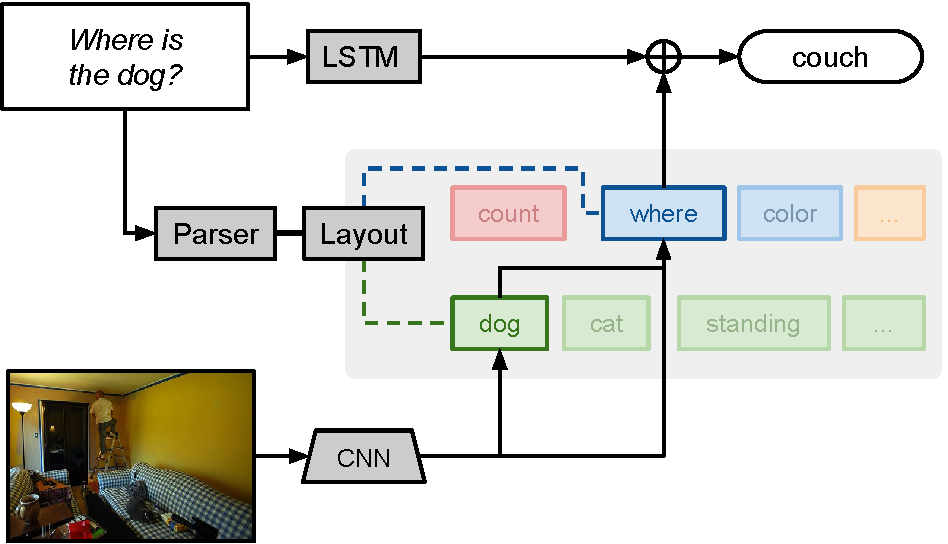
\includegraphics[width=\linewidth]{fig/teaser}
\end{center}
   \caption{Our approach answers questions about images, it automatically instantiates different modules of neural networks depending on the question. An additional LSTM provides sentence context and learns common sense / dataset bias.}
\label{fig:teaser}
\end{figure}
% how is this different from previous work? ack mateusz and jayant
% what is the problem?
Answering natural language questions about images is an interesting task, as it has many applications in human-robot interaction such as assisting blind people. However, it is also an important research direction as it requires to combine fundamental techniques in both computer vision and natural language processing and has recently received increased attention in the computer vision and natural language processing communities \cite{antol15iccv,gao2015you,ma15arxiv,malinowski15iccv,ren2015image,yu15arxiv}.

Specifically, the problem we approach in this paper is given a natural language question, \eg \emph{Where is the dog?}, and an image we want to predict an an answer, \eg \emph{on the couch}. 
Recent successful approaches for answering questions about images, represent questions as bag-of-words \cite{} or read in the question using a single recurrent neural network (RNN) \cite{malinowski15iccv}\cite{} and train a classifier on the full sentence representation and the full-image convolutional neural network (CNN). 
Another line of work  \cite{malinowski15nips} uses semantic parsers from the natural language processing
literature to decompose questions into logical expressions which are evaluated with respect to the image content.

In this paper we want to draw from these two different direction and presents a general-purpose technique for integrating the
representational power of neural networks with the flexible compositional
structure afforded by symbolic approaches to semantics. 
Specifically we propose a novel architecture, \nmn (NMN), where several neural network components or ``modules'' are discretely composed together in a deep network based on a semantic structure, but trained jointly across examples.  Specifically, for question answering we visualize our approach in \Figref{fig:teaser}. We parse the question with a semantic parser to decompose it into its main components \ldots [describe Figure].
Importantly, all modules of a NMN are independent, which allows the computation to be different for each problem instance, and does not need to be observed during training. So that we can answer novel question at test time, such as \emph{Where is the banana?}, even we only saw \emph{count} or \emph{color} question about \emph{bananas} during training.

\todo{One or two sentences of potential other use cases of NMNs?}

% Where previous work has
%treated both the image and the question as inputs to a monolithic classification
%model, we instead take the perspective that a question is a noisy specification
%of a hidden computation that must be performed on the image to produce an
%answer. Crucially, this computation may be different for each problem instance,
%and is never observed observed during training.

%Our approach bears a superficial resemblance to a classical semantic parser.
%However, instead of mapping from questions to logical forms, our model maps from
%questions to neural network structures. These networks are assembled on the fly
%(possibly into novel topologies) from a collection of jointly-learned neural
%``modules''. Finally, they are evaluated against the input image to produce an
%answer.




%This paper presents a technique for following natural language instructions (and
%performing other dynamically-specified tasks) by assembling deep neural networks
%on the fly from an inventory of pre-trained components.

We evaluate our approach on three visual question answering tasks. On the
recently-released CocoQA and VQA datasets, we achieve results comparable to
[better than] existing approaches, and show that our approach specifically outperforms
previous work on questions with compositional structure [e.g. requiring that an
object be located and one of its attributes described]. However, most of the
questions in both datasets are quite simple, involving little or no composition.
To test our approach's ability to handle highly structured questions, we
introduce a new dataset of synthetic images paired with complex questions
involving spatial relations, logical operators, and shape and attribute
recognition. On this dataset we outperform the previous state of the art by XXX.

%We evaluate our approach on two visual question answering tasks. First we
%present a new synthetic image dataset paired with a complex set of queries
%(involving spatial relations, logical operators, and shape and
%attribute recognition). Next, we consider a hard subset of the Microsoft VQA
%corpus of questions about natural images. In each case, an NMN-based approach
%outperforms state-of-the-art models with more conventional recurrent
%architectures. We observe in particular that NMNs are able to make considerably
%better use of small training sets.

The contributions of this work are as follows. First, we propose a novel architecture \nmn (NMN), which consist of composable neural
modules which can be composed to deep networks, are trained jointly across modules, and allow to be assembled into novel topologies at evaluation time.
Second, for answering question about images we show how to construct NMNs based on a semantic parser output, and jointly trained with a CNN image representation and a LSTM question representation to succesfully answer questions. 
Third, we provide a thorough experimental evaluation on three datasets, providing insides on different realizations of NMNs.
Finally, we will release our code and experimental setup, as well as the synthetic QA dataset upon publication.
%First, we demonstrate
%technique for using
%that off-the-shelf tools for linguistic structure prediction can be used to
%inform decisions about neural network structure. Second, and more
%generally, we demonstrate that it is possible to train a collection of composable neural
%modules in such a way that they can be assembled into novel topologies at
%evaluation time.

In the following we first\ldots  [Outline]